%% Template for MLP Coursework 1 / 19 October 2021 

%% Based on  LaTeX template for ICML 2017 - example_paper.tex at 
%%  https://2017.icml.cc/Conferences/2017/StyleAuthorInstructions

\documentclass{article}
\usepackage[T1]{fontenc}
\usepackage{amssymb,amsmath}
\usepackage{txfonts}
\usepackage{microtype}

% For figures
\usepackage{graphicx}
\usepackage{subcaption} 

% For citations
\usepackage{natbib}

% For algorithms
\usepackage{algorithm}
\usepackage{algorithmic}

% the hyperref package is used to produce hyperlinks in the
% resulting PDF.  If this breaks your system, please commend out the
% following usepackage line and replace \usepackage{mlp2017} with
% \usepackage[nohyperref]{mlp2017} below.
\usepackage{hyperref}
\usepackage{url}
\urlstyle{same}

\usepackage{color}
\usepackage{booktabs} % To thicken table lines
\usepackage{multirow} % Multirow cells in table

% Packages hyperref and algorithmic misbehave sometimes.  We can fix
% this with the following command.
\newcommand{\theHalgorithm}{\arabic{algorithm}}


% Set up MLP coursework style (based on ICML style)
\usepackage{mlp2021}
\mlptitlerunning{MLP Coursework 1 (\studentNumber)}
\bibliographystyle{icml2017}
\usepackage{bm,bbm}


\DeclareMathOperator{\softmax}{softmax}
\DeclareMathOperator{\sigmoid}{sigmoid}
\DeclareMathOperator{\sgn}{sgn}
\DeclareMathOperator{\relu}{relu}
\DeclareMathOperator{\lrelu}{lrelu}
\DeclareMathOperator{\elu}{elu}
\DeclareMathOperator{\selu}{selu}
\DeclareMathOperator{\maxout}{maxout}
\newcommand{\bx}{\bm{x}}




\definecolor{red}{rgb}{0.95,0.4,0.4}
\definecolor{blue}{rgb}{0.4,0.4,0.95}
\definecolor{orange}{rgb}{1, 0.65, 0}

\newcommand{\youranswer}[1]{{\color{red} \bf[#1]}} %your answer: 


%% START of YOUR ANSWERS
%% REPLACE sXXXXXXX with your student number
\def\studentNumber{sXXXXXXX}


%% START of YOUR ANSWERS
%% Add answers to the questions below, by replacing the text inside the brackets {} for \youranswer{ "Text to be replaced with your answer." }. 
%
% Do not delete the commands for adding figures and tables. Instead fill in the missing values with your experiment results, and replace the images with your own respective figures.
%
% You can generally delete the placeholder text, such as for example the text "Question Figure 2 - Replace the images ..." 
%
% There are 19 TEXT QUESTIONS (a few of the short first ones have their answers added to both the Introduction and the Abstract). Replace the text inside the brackets of the command \youranswer with your answer to the question.
%
% There are also 3 "questions" to replace some placeholder FIGURES with your own, and 3 "questions" asking you to fill in the missing entries in the TABLES provided. 
%
% NOTE! that questions are ordered by the order of appearance of their answers in the text, and not by the order you should tackle them. Specifically, you cannot answer Questions 2, 3, and 4 before concluding all of the relevant experiments and analysis. Similarly, you should fill in the TABLES and FIGURES before discussing the results presented there. 
%
% NOTE! If for some reason you do not manage to produce results for some FIGURES and TABLES, then you can get partial marks by discussing your expectations of the results in the relevant TEXT QUESTIONS (for example Question 8 makes use of Table 1 and Figure 2).
%
% Please refer to the coursework specification for more details.


%% - - - - - - - - - - - - TEXT QUESTIONS - - - - - - - - - - - - 

%% Question 1:
\newcommand{\questionOne} {
\youranswer{the phenomenon that occurs when a model's predictions align too closely to its limited training set, reducing it ability to generalise to unseen data}
}

%% Question 2:
\newcommand{\questionTwo} {
\youranswer{Question 2 - Summarise the effect increasing width and depth of the architecture had on overfitting}
}

%% Question 3:
\newcommand{\questionThree} {
\youranswer{Question 3 - Summarise what your results show you about the effect of the tested approaches on overfitting and the performance of the trained model}
}

%% Question 4:
\newcommand{\questionFour} {
\youranswer{Question 4 - Give your overall conclusions}
}

%% Question 5:
\newcommand{\questionFive} {
\youranswer{Question 5 - Explain what overfitting is in detail and in your own words}
}

%% Question 6:
\newcommand{\questionSix} {
\youranswer{Question 6 - Discuss ``why'' and ``how'' overfitting occurs, and ``how'' one can identify it is happening}
}

%% Question 7:
\newcommand{\questionSeven} {
\youranswer{Question 7 - Explain what these figures contain and how the curves evolve, and spot where overfitting occurs. Reason based on the min/max points and velocities (direction and magnitude of change) of the accuracy and error curves}
}

%% Question 8:
\newcommand{\questionEight} {
\youranswer{Question 8 - Explain your network width experiment results by using the relevant figure and table}
}

%% Question 9:
\newcommand{\questionNine} {
\youranswer{Question 9 - Discuss whether varying width affects the results in a consistent way, and whether the results are expected and match well with the prior knowledge (by which we mean your expectations as are formed from the relevant Theory and literature)}
}

%% Question 10:
\newcommand{\questionTen} {
\youranswer{Question 10 - Explain your network depth experiment results by using the relevant figure and table}
}

%% Question 11:
\newcommand{\questionEleven} {
\youranswer{Question 11 - Discuss whether varying depth affects the results in a consistent way, and whether the results are expected and match well with the prior knowledge (by which we mean your expectations as are formed from the relevant Theory and literature)}
}

%% Question 12:
\newcommand{\questionTwelve} {
\youranswer{Question 12 - Compare and discuss how varying width and height changes the performance and overfitting in your experiments}
}

%% Question 13:
\newcommand{\questionThirteen} {
\youranswer{Question 13 - Explain L1/L2 weight penalties first in words and then with formulas. Explain how they are incorporated to training and what hyperparameter(s) they require}
}

%% Question 14:
\newcommand{\questionFourteen} {
\youranswer{Question 14 - Discuss how/why the weight penalties may address overfitting, discuss how L1 and L2 regularization differ and support your claims with references where possible}
}

%% Question 15:
\newcommand{\questionFifteen} {
\youranswer{Question 15 - Explain the experimental details (e.g. hyperparameters), discuss the results in terms of their generalization performance and overfitting}
}

%% Question 16:
\newcommand{\questionSixteen} {
\youranswer{Question 16 - Explain the motivation behind Maxout Networks as presented in \cite{goodfellow2013maxout}
}
}

%% Question 17:
\newcommand{\questionSeventeen} {
\youranswer{Question 17 - State whether Dropout is compatible (can be used together) with Maxout and explain why
}
}

%% Question 18:
\newcommand{\questionEighteen} {
\youranswer{Question 18 - Give an overview of the experiment setup in \cite{goodfellow2013maxout} and analyse it from the point of view of how convincing their conclusions are 
}
}

%% Question 19:
\newcommand{\questionNineteen} {
\youranswer{Question 19 - Briefly draw your conclusions based on the results from the previous sections (what are the take-away messages?) and conclude your report with a recommendation for future directions
}
}


%% - - - - - - - - - - - - FIGURES - - - - - - - - - - - - 

%% Question Figure 2:
\newcommand{\questionFigureTwo} {
\youranswer{Question Figure 2 - Replace the images in Figure 2 with figures depicting the accuracy and error, training and validation curves for your experiments varying the number of hidden units.

\begin{figure}[t]
    \centering
    \begin{subfigure}{\linewidth}
        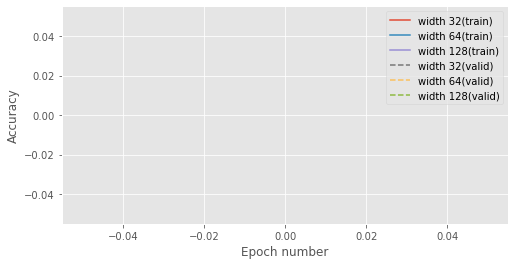
\includegraphics[width=\linewidth]{figures/empty_acc_curve_width.png}
        \caption{accuracy by epoch}
        \label{fig:width_acccurves}
    \end{subfigure} 
    \begin{subfigure}{\linewidth}
        \centering
        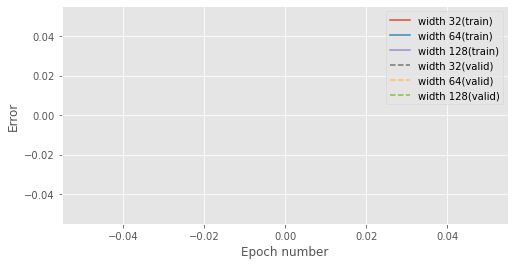
\includegraphics[width=\linewidth]{figures/empty_error_curve_width.png}
        \caption{error by epoch}
        \label{fig:width_errorcurves}
    \end{subfigure} 
    \caption{Training and validation curves in terms of classification accuracy (a) and cross-entropy error (b) on the EMNIST dataset for different network widths.}
    \label{fig:width}
\end{figure} 

}
}

%% Question Figure 3:
\newcommand{\questionFigureThree} {
\youranswer{Question Figure 3 - Replace these images with figures depicting the accuracy and error, training and validation curves for your experiments varying the number of hidden layers.

\begin{figure}[t]
    \centering
    \begin{subfigure}{\linewidth}
        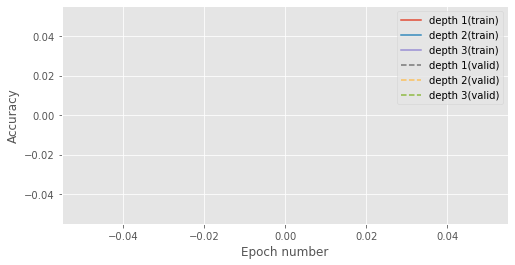
\includegraphics[width=\linewidth]{figures/empty_acc_curve_depth.png}
        \caption{accuracy by epoch}
        \label{fig:depth_acccurves}
    \end{subfigure} 
    \begin{subfigure}{\linewidth}
        \centering
        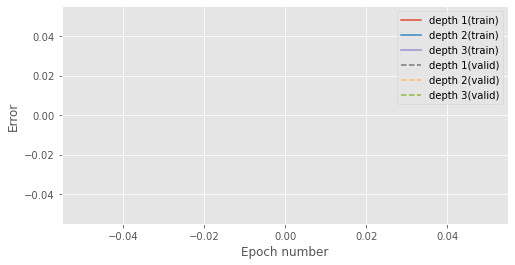
\includegraphics[width=\linewidth]{figures/empty_error_curve_depth.png}
        \caption{error by epoch}
        \label{fig:depth_errorcurves}
    \end{subfigure} 
    \caption{Training and validation curves in terms of classification accuracy (a) and cross-entropy error (b) on the EMNIST dataset for different network depths.}
    \label{fig:depth}
\end{figure} 

}
}

%% Question Figure 4:
\newcommand{\questionFigureFour} {
\youranswer{Question Figure 4 - Replace these images with figures depicting the Validation Accuracy and Generalisation Gap for each of your experiments varying the Dropout rate, L1/L2 weight penalty, and for the 8 combined experiments (you will have to find a way to best display this information in one subfigure).

\begin{figure*}[t]
    \centering
    \begin{subfigure}{.3\linewidth}
        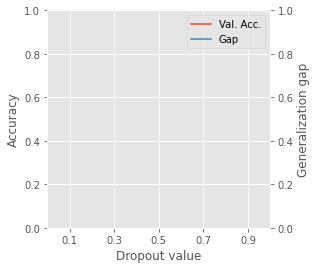
\includegraphics[width=\linewidth]{figures/empty_dropout_plot.png}
        \caption{Metrics by dropout rate}
        \label{fig:dropoutrates}
    \end{subfigure} 
    \begin{subfigure}{.3\linewidth}
        \centering
        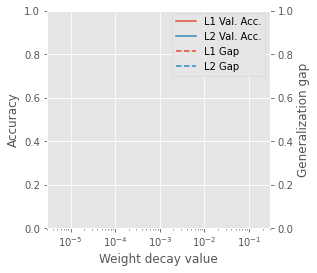
\includegraphics[width=\linewidth]{figures/empty_wd_plot.png}
        \caption{Metrics by weight penalty}
        \label{fig:weightrates}
    \end{subfigure} 
    \begin{subfigure}{.3\linewidth}
        \centering
        \includegraphics[width=.85\linewidth]{example-image-duck}
        \caption{Extra experiments}
        \label{fig:extra}
    \end{subfigure} 
    \caption{Hyperparameter search for every method and combinations}
    \label{fig:hp_search}
\end{figure*}

}
}

%% - - - - - - - - - - - - TABLES - - - - - - - - - - - - 

%% Question Table 1:
\newcommand{\questionTableOne} {
\youranswer{
Question Table 1 - Fill in Table 1 with the results from your experiments varying the number of hidden units.

\begin{table}[t]
    \centering
    \begin{tabular}{c|cc}
    \toprule
        \# hidden units & val. acc. & generalization gap \\
    \midrule
         32            &            &                    \\
         64            &            &                    \\
         128           &            &                    \\ 
    \bottomrule
    \end{tabular}
    \caption{Validation accuracy (\%) and generalization gap (in terms of cross-entropy error) for varying network widths on the EMNIST dataset.}
    \label{tab:width_exp}
\end{table}
}
}

%% Question Table 2:
\newcommand{\questionTableTwo} {
\youranswer{
Question Table 2 - Fill in Table 2 with the results from your experiments varying the number of hidden layers.

\begin{table}[t]
    \centering
    \begin{tabular}{c|cc}
    \toprule
        \# hidden layers & val. acc. & generalization gap \\
    \midrule
         1               &            &                    \\
         2               &            &                    \\
         3               &            &                    \\ 
    \bottomrule
    \end{tabular}
    \caption{Validation accuracy (\%) and generalization gap (in terms of cross-entropy error) for varying network depths on the EMNIST dataset.}
    \label{tab:depth_exps}
\end{table}
}
}

%% Question Table 3:
\newcommand{\questionTableThree} {
\youranswer{
Question Table 3 - Fill in Table 3 with the results from your experiments varying the hyperparameter values for each of L1 regularisation, L2 regularisation, and Dropout (use the values shown on the table) as well as the results for your experiments combining L1/L2 and Dropout (you will have to pick what combinations of hyperparameter values to test for the combined experiments; each of the combined experiments will need to use Dropout and either L1 or L2 regularisation; run an experiment for each of 8 different combinations). Use \textit{italics} to print the best result per criterion for each set of experiments, and \textbf{bold} for the overall best result per criterion.

\begin{table*}[t]
    \centering
    \begin{tabular}{c|c|cc}
    \toprule
        Model    &  Hyperparameter value(s) & Validation accuracy & Generalization gap \\
    \midrule
    \midrule
        Baseline &  -                    &                     &                   \\
    \midrule
        \multirow{5}*{Dropout}
                 & 0.1                   &                     &                   \\
                 & 0.3                   &                     &                   \\
                 & 0.5                   &                     &                   \\
                 & 0.7                   &                     &                   \\
                 & 0.9                   &                     &                   \\
    \midrule
        \multirow{5}*{L1 penalty}
                 & 1e-5                   &                     &                   \\
                 & 1e-4                   &                     &                   \\
                 & 1e-3                   &                     &                   \\
                 & 1e-2                   &                     &                   \\
                 & 1e-1                   &                     &                   \\
    \midrule
        \multirow{5}*{L2 penalty}  
                 & 1e-5                   &                     &                   \\
                 & 1e-4                   &                     &                   \\
                 & 1e-3                   &                     &                   \\
                 & 1e-2                   &                     &                   \\
                 & 1e-1                   &                     &                   \\
    \midrule
        \multirow{8}*{Combined}  
                 & for example 0.95, L1 1e-6  &                     &                   \\
                 & ?, ?                   &                     &                   \\
                 & ?, ?                   &                     &                   \\
                 & ?, ?                   &                     &                   \\
                 & ?, ?                   &                     &                   \\
                 & ?, ?                   &                     &                   \\
                 & ?, ?                   &                     &                   \\
                 & ?, ?                   &                     &                   \\
    \bottomrule
    \end{tabular}
    \caption{Results of all hyperparameter search experiments. \emph{italics} indicate the best results per series and \textbf{bold} indicate the best overall}
    \label{tab:hp_search}
\end{table*}

}
}

%% END of YOUR ANSWERS
%% END of YOUR ANSWERS



%% Do not change anything in this file. Add your answers to mlp-cw1-questions.tex



\begin{document} 

\twocolumn[
\mlptitle{MLP Coursework 1}
\centerline{\studentNumber}
\vskip 7mm
]

\begin{abstract} 
In this report we study the problem of overfitting, which is \questionOne.
We first analyse the given example and discuss the probable causes of the underlying problem. 
Then we investigate how the depth and width of a neural network
can affect overfitting in a feedforward architecture and observe that increasing width and depth \questionTwo.
Next we discuss why two standard methods, Dropout and Weight Penalty, can
mitigate overfitting, then describe their implementation and use them in our experiments
to reduce the overfitting on the EMNIST dataset. 
Based on our results, we ultimately find that \questionThree.
Finally, we briefly review another method, Maxout, discuss its strengths and weaknesses, and conclude the report with our observations and future work. Our main findings indicate that \questionFour.
\end{abstract} 

\section{Introduction}
\label{sec:intro}
In this report we focus on a common and important problem while training machine learning models known as overfitting, or overtraining, which is \questionOne.
We first start with analyzing the given problem in Fig.~\ref{fig:example}, study it in different architectures and then investigate different strategies to mitigate the problem.
In particular, Section \ref{sec:task1} identifies and discusses the given problem, and investigates the effect of network width and depth in terms of generalization gap (see Ch.~5 in \citealt{Goodfellow-et-al-2016}) and generalization performance.
Section \ref{sec:task2.1} introduces two regularization techniques to alleviate overfitting: Dropout \cite{srivastava2014dropout} and L1/L2 Weight Penalties (see Section~7.1 in \citealt{Goodfellow-et-al-2016}). 
We first explain them in detail and discuss why they are used for alleviating overfitting.
In Section~\ref{sec:task2.2} we incorporate each of them and their various combinations to a three hidden layer neural network, train it on the EMNIST dataset, which contains 131,600 images of characters and digits, each of size 28x28 which are split into 47 classes, grouping together some difficult to distinguish characters.
We evaluate them in terms of generalization gap and performance, and discuss the results and effectiveness of the tested regularization strategies.
Our results show that \questionThree.
In Section~\ref{sec:task3}, we discuss a related work on Maxout Networks and highlight its pros and cons.\footnote{Instructor note: Omitting this for this coursework, but normally you would be more specific and summarise your conclusions about that review here as well.}
Finally, we conclude our study in section \ref{sec:concl}, noting that \questionFour.


\section{Problem identification}
\label{sec:task1}

\begin{figure}[t]
    \centering
    \begin{subfigure}{\linewidth}
        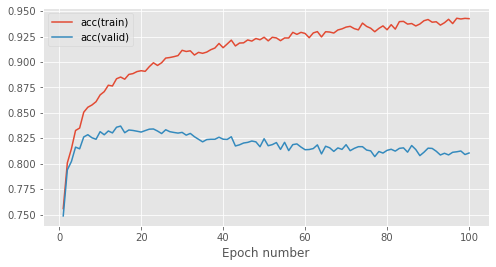
\includegraphics[width=\linewidth]{figures/accuracy_IHO_withrelu.png}
        \caption{accuracy by epoch}
        \label{fig:example_acccurves}
    \end{subfigure} 
    \begin{subfigure}{\linewidth}
        \centering
        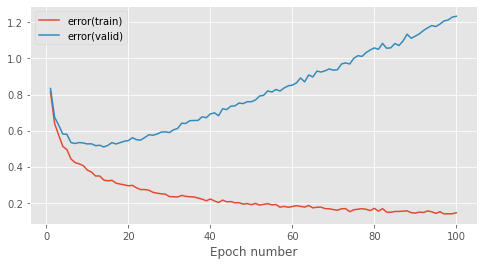
\includegraphics[width=\linewidth]{figures/error_IHO_withrelu.png}
        \caption{error by epoch}
        \label{fig:example_errorcurves}
    \end{subfigure} 
    \caption{Training and validation curves in terms of classification accuracy (a) and cross-entropy error (b) on the EMNIST dataset for the baseline model.}
    \label{fig:example}
\end{figure} 

Overfitting to training data is a very common and important issue that needs to be dealt with when training neural networks or other machine learning models in general (see Ch.~5 in \citealt{Goodfellow-et-al-2016}).
A model is said to be overfitting when \questionFive.

\questionSix.

Fig.~\ref{fig:example_acccurves} and \ref{fig:example_errorcurves} show a prototypical example of overfitting.
We see in Figure~\ref{fig:example_acccurves} that \questionSeven.

The extent to which our model overfits depends on many factors.
For example, the quality and quantity of the training set and
the complexity of the model. If we have a lot of varied training samples,
or if our model is relatively shallow, it will in general
be less prone to overfitting. Any form of regularisation
will also limit the extent to which the model overfits.


\subsection{Network width}

\questionTableOne
\questionFigureTwo


First we investigate the effect of increasing the number of
hidden units in a single hidden layer network when training
on the EMNIST dataset.
The network is trained using the Adam optimizer
with a learning rate of $10^{-3}$ and a batch size of 100, for a total of 100 epochs.


The input layer is of size 784, and output layer consists
of 47 units. 
Three different models were trained, with a
single hidden layer of 32, 64 and 128 ReLU hidden units
respectively.
Figure~\ref{fig:width} depicts the error and accuracy curves over 100 epochs for the model with varying number of hidden units.
Table~\ref{tab:width_exp} reports the final accuracy and generalization gap.
We observe that \questionEight.

\questionNine.


\subsection{Network depth}

\questionTableTwo
\questionFigureThree

Next we investigate the effect of varying the number of hidden
layers in the network. 
Table~\ref{tab:depth_exps} and Fig.~\ref{fig:depth} shows the results from
training three models with one, two and three hidden layers respectively,
each with 128 ReLU hidden units. 
As with previous experiments, they are 
trained with the Adam optimizer with a learning rate of  $10^{-3}$ and 
a batch size of 100. 

We observe that \questionTen.

\questionEleven.

\questionTwelve.





\section{Dropout and Weight Penalty}
\label{sec:task2.1} 

In this section, we investigate three regularization methods to 
alleviate the overfitting problem, specifically dropout layers 
and the L1 and L2 weight penalties.

\subsection{Dropout}

Dropout~\cite{srivastava2014dropout}
is a stochastic method that randomly inactivates
neurons in a neural network according to an hyperparameter, the
dropout rate. Dropout is commonly represented by an 
additional layer inserted between the linear layer and 
activation function.
Its forward propagation during training is defined as follows:

\begin{align}
    mask &\sim bernoulli(p)\\
    y' &= mask \odot y\
\end{align}

where $y, y' \in \mathbb{R}^d$ are the output of the linear layer 
before and after applying dropout, 
respectively. $mask \in \mathbb{R}^d$ is a mask vector randomly sampled from the
Bernoulli distribution with parameter of inclusion probability
$p$, and $\odot$ denotes the element-wise multiplication.

At inference time, stochasticity is not desired, so no neurons
are dropped. To account for the change in expectations of the
output values, we scale them down by the inclusion rate
$p$:

\begin{align}
    y' &= y*p\
\end{align}

As there is no nonlinear calculation involved, the backward
propagation is just the element-wise product of the gradients
with respect to the layer outputs and mask created
in the forward calculation. The backward propagation for
dropout is therefore formulated as follows:

\begin{align}
    \frac{\partial y'}{\partial y} = mask
\end{align}

Dropout is an easy to implement and highly scalable
method. It can be implemented as a layer-based calculation
unit, and be placed on any layer of the neural network at
will. Dropout can reduce the dependence of hidden features
between layers so that the neurons of the next layer will not
specifically depend on some features from of the previous layer.
Instead, it force the network to evenly distribute information
among all features. By randomly dropping some neurons in training,
dropout makes use of a subset of the whole architecture, so it can 
also be viewed as bagging different sub networks and averaging their
outputs.



\subsection{Weight penalty}

L1 and L2 regularization~\cite{ng2004feature} are simple but effective
methods to mitigate overfitting to training data.
\questionThirteen.

\questionFourteen.



\section{Balanced EMNIST Experiments}

\questionTableThree

\questionFigureFour

\label{sec:task2.2}

Here we evaluate the effectiveness of the given regularization methods for reducing the overfitting on the EMNIST dataset.
We build a baseline architecture with three hidden layers, each with 128 neurons, which suffers from overfitting in EMNIST as shown in section \ref{sec:task1}.
We follow the previous training settings where we deliberately let the baseline overfit
on the training set as in previous experiments. 
These settings ensure the fairness of the evaluation of three methods to alleviate overfitting. 
Then, we apply the L1 or L2 regularization with dropout to our baseline and search for good hyperparameters on the validation set. 
We summarize all
the experimental results in Table~\ref{tab:hp_search}. For each method, we
plot the relationship between generalisation gap and validation accuracy in Figure~\ref{fig:hp_search}.

First we analyze three methods separately, train each over a set of hyperparameters and compare their best performing results.

\questionFifteen.


\section{Literature Review: Maxout Networks}
\label{sec:task3}

\paragraph{Summary of Maxout Networks} In this section, we
briefly discuss another generalization method: Maxout net-
works \cite{goodfellow2013maxout}. This paper further ex-
plores the dropout method and proposes a new "maxout" layer
 which can complement dropout.
The authors evaluate the performance of Maxout Networks
in four standard datasets, namely MNIST, CIFAR-10
and 100, and SVHN. They point out that although
dropout has been widely applied in deep models, \questionSixteen. Following this 
motivation, they propose the Maxout activation layers. These can be considered learnable activations that work as a universal convex function approximator. The Maxout layer first
maps the hidden space to $k$ subspaces through independent
affine transformations, then, for each element in output
vectors, it takes the maximum value across all subspaces.

\questionSeventeen.

\paragraph{Strengths and limitations} The author proposed a novel
neural activation unit that further exploits the dropout technique.
\questionEighteen.

Although the Maxout activation units can maximize
the averaging effect of dropout in a deep architecture,
we can argue that the Maxout computation
is expensive. The advantage of dropout lies in its high 
scalability and computational advantages. It can be arbitrarily
applied to various network structures, and the calculation
speed is fast, which is very suitable for heavy computing 
algorithms such as training and inference of neural networks.
In comparison, the design of the Maxout network needs to project the
hidden vector into $k$ subspaces. Both the forward algorithm and the
backward algorithm of dropout can be calculated in $\mathcal{O}(D)$
complexity, but the complexity of Maxout is $\mathcal{O}(kD)$.
This can lead to increasing the number of training epochs needed
to reach convergence. 
Furthermore, the universal approximation property of Maxout seems
powerful, but it would be interesting to verify that it is useful
in practice. Specifically, we can design an experiment where we 
increase the number of subspaces $k$ and see where performances stop
improving. In extreme cases, it is even possible that the 
function learned is too specific to the training data, effectively
causing overfitting.



\section{Conclusion}
\label{sec:concl}
    
\questionNineteen.

\bibliography{refs}

\end{document} 

